\chapter{Konzeption}

In diesem Kapitel wird die Konzeption des Gesamtsystems beschrieben. Es wird die Nutzungskontextanalyse beschrieben, welches als Grundlage und Vorbereitung für die anschließende Anforderungsanalyse diente. Die Anforderungsanalyse in welcher, im Rahmen eines Kreativ Workshops, Anwendungsfälle für das zu konzipierende System erarbeitet wurden, wird erläutert. Abschließend wird einEntwurf der Anwendung beschrieben.

\section{Nutzungskontextanalyse}

% Aktuelle Problemlösungstrategien? Bewertungen auf Online Portalen, Blogs, Interessengruppen, Reklamationen, Technischer Support
Aktuelle Lösungen für die Abgabe von Rückmeldungen zur Gestaltung von Produkten erfolgt oft ohne den Einsatz von Augmented Reality. Diese erfolgen 
oft als Bewertungen in Online Einkaufsportalen, Blog Beiträgen, durch den Austausch in Interessengruppen oder über direkten Kontakt zum Hersteller, die 
meist über die Kontaktaufnahme zum technischen Support erfolgt.

Bei Bewertungen in Onlineportalen, in Blog Beiträgen oder auch bei direktem Kontakt zum Hersteller (z.Bsp. durch E-Mail), haben Kunden die Möglichkeit 
ihre Gestaltungsidee schriftlich zu beschreiben und mit Bildern oder Videos zu ergänzen. Bei solchen Beschreibungen kommt es jedoch manchmal vor dass 
nicht immer klar hervorgeht zu welcher Stelle oder zu welchem Teil am Produkt sich die Beschreibung bezieht. Die Umgebung als Kontext in welchem das Produkt 
verwendet wird geht aus solchen Beschreibungen nicht immer hervor. Zudem ist nicht ohne Aufwand möglich direkt zu erkennen an welchen Stellen eines Produktes 
welche Rückmeldungen häufen. \footnote{Z.Bsp.: Angenommen es gibt zum Produkt sehr viele unterschiedliche Rückmeldungen. Mit direktem Blick zu erkennen dass sich
die meisten Rückmeldungen bei einem Produkt  (z. Bsp. einer Kaffeetasse) auf die untere Kante am Griff beziehen.} 

Bei Interessengruppen in welchen Nutzer von bestimmten Produkten, sich an einem Ort treffen um Erfahrungen auszutauschen wie z.Bsp. bei Hausaltprodukten, Modellflugzeugen, VR Brillen etc., 
haben die Nutzer die Möglichkeit ihre Ideen genauer zu beschreiben. Bei solchen Treffen haben die Nutzer die Möglichkeit mit Bezugnahme auf die Stellen am Produkt und dem Kontext 
ihrer Umgebung zu ihre Ideen zu beschreiben. Das Problem bei dieser Art der Rückmeldungen ist jedoch dessen eingrenzte Reichweite. Zudem werden Inhalte welche in solchen Treffen diskutiert 
wurden oft nicht ausreichend dokumentiert.  

Auf Basis der im Kapitel \ref{CapterFundamentals} behandelten Grundlagen und der Nutzungskontextanalyse wurde eine erste Skizze des Gesamtsystems entworfen in welcher, 
Funktionale wie Nicht-Funktionale Anforderungen an das zu konzipierende System skizziert wird (siehe Abbildung \ref{img:sysstem_sketch}).

\begin{figure}[H]
	\centering
	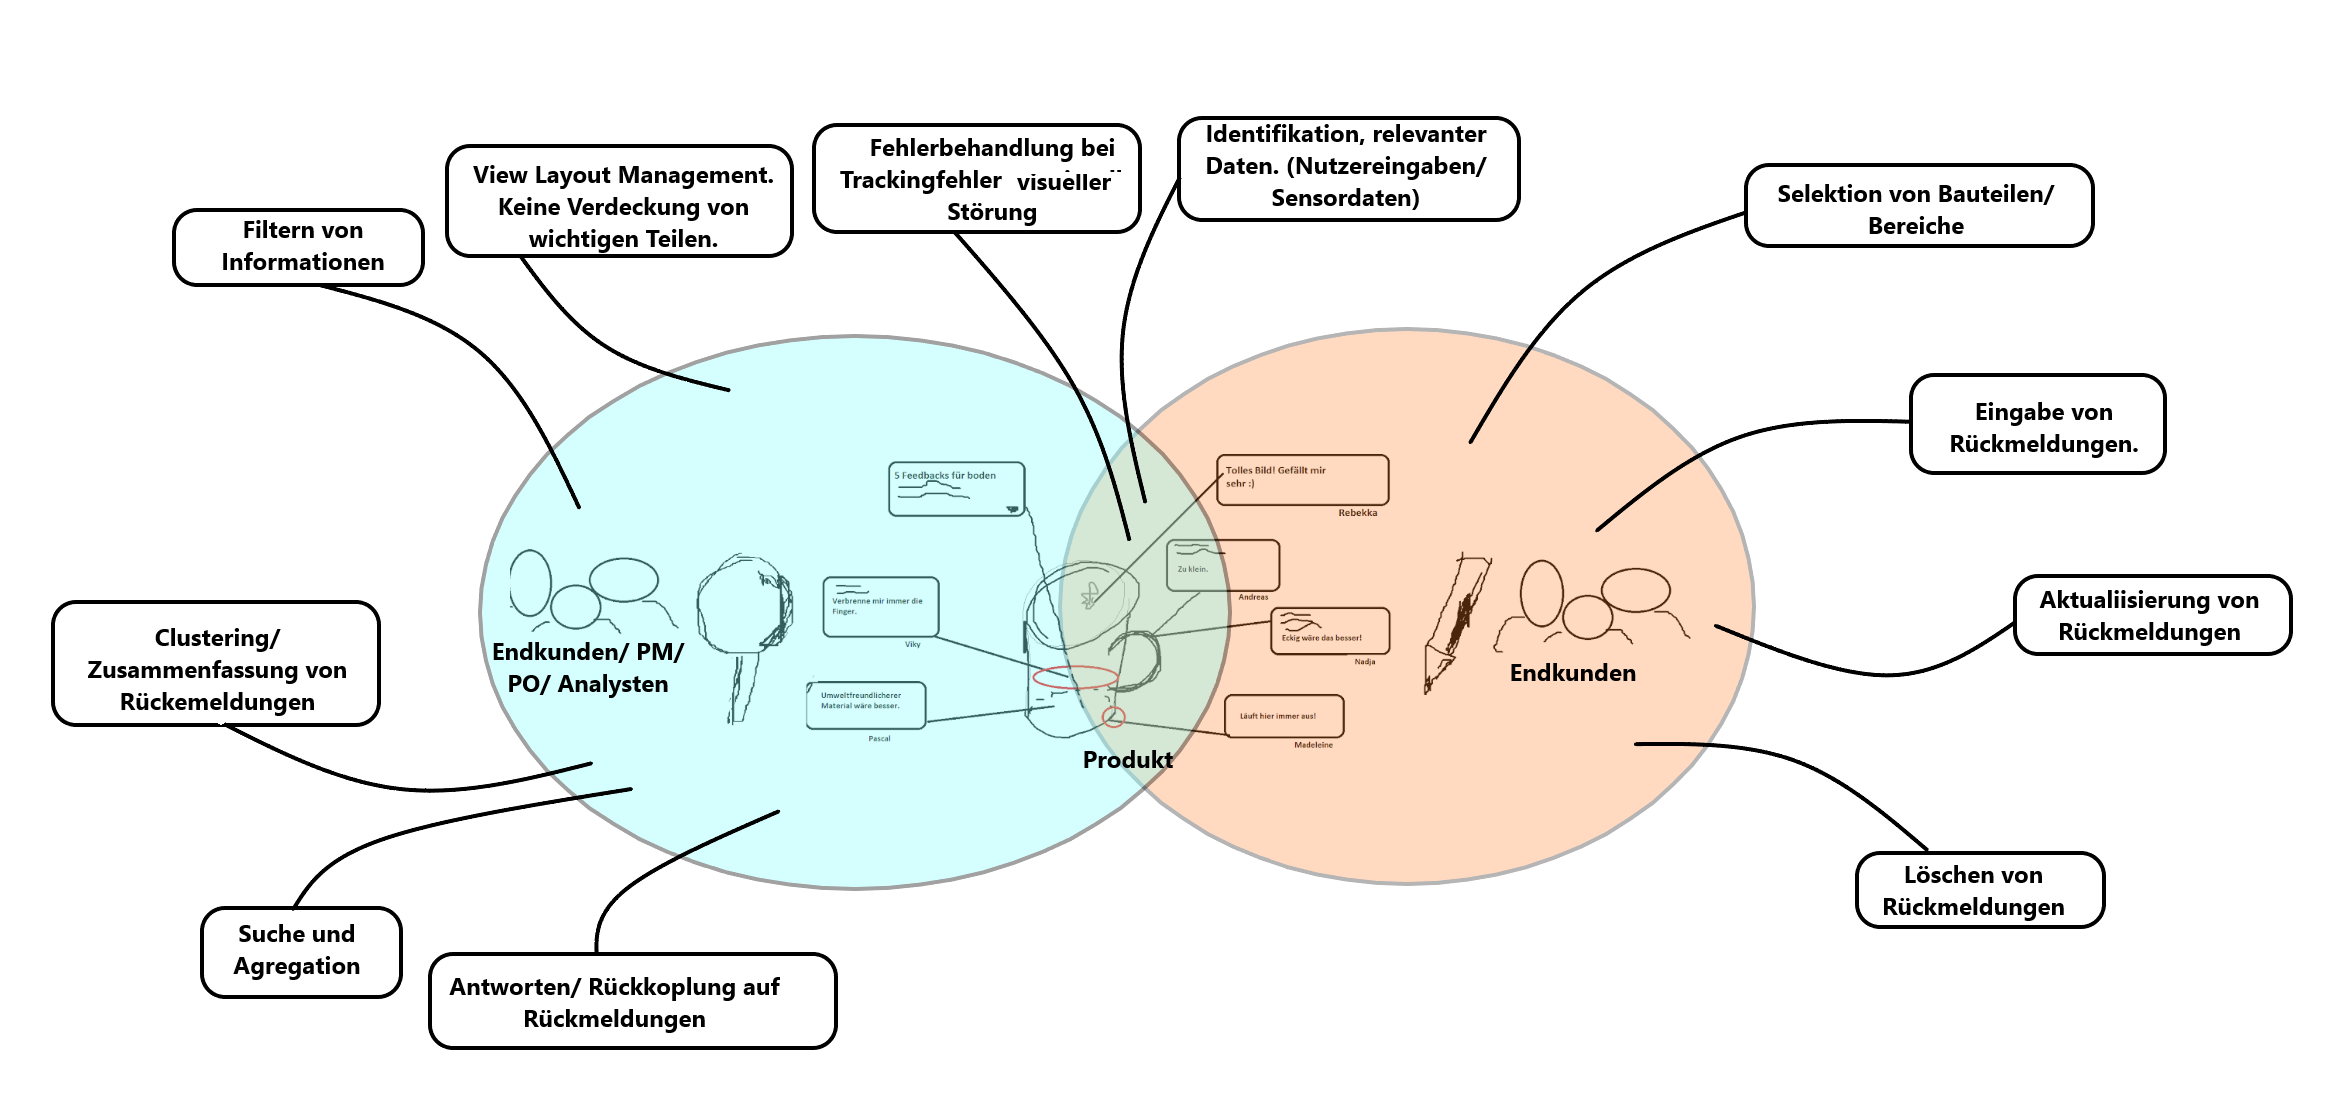
\includegraphics[width=1.0\textwidth]{resources/conception/skizze_gesamtsystem.png}
	\caption{Skizze des Gesamtsystems als erster Entwurf \cite{system sketch}}
	\label{img:sysstem_sketch}
\end{figure}

Dieses Skizze sollte die Projektidee begreifbarer machen und als grobe Orientierung bei der Anforderungsanalyse dienen.

\section{Anforderungsanalyse}

Die Anforderungsanalyse wurde im Rahmen eines Kreativ Workshops durchgeführt. Ziel des Workshops war es Die Nutzer für das zu konzipierende System zu identifizieren und deren Eigenschaften und Bedürfnisse 
zu analysieren. 

% Vorbereitung
Das Workshop fand am dritten Juli, am Fraunhofer IPK in Berlin statt. Zur Vorbereitung wurde in einem zuvor für diesen Workshop gebuchten, Besprechungsraum, einzelne Stationen \footnote{z.Bsp.: Pinnwand, Kärtchen, Abbildungen Personen für die Erstellung von Personas usw.} für die am Workshop durchzuführenden Aktivitäten vorbereitet. 
Zunächst wurden die Teilnehmer begrüßt, der Anlass und der Ablauf des Workshop erklärt und die Teilnahme am Workshop bedankt. 

%Durchführung
Mit Hilfe einer kurzen Power-Point Präsentation wurde die Projektidee vorgestellt und anhand der groben Skizze des zu konzipierenden Systems (Abbildung \ref{img:sysstem_sketch}) verdeutlicht. 
Anschließend fand eine Frage- Antwort Runde statt, welches die Möglichkeit gab, Rückfragen zu stellen und somit sicherzustellen, dass die Projektidee von jedem Teilnehmer gleichermaßen verstanden wurde. 

Nach der Vorstellung der Projektidee fand ein Brainstorming statt, dessen Ergebnis in ein Affinitätsdiagramm festgehalten wurde. 
Im gewöhnlichen Vorgang für die Erstellung von Affinitätsdiagrammen, schreiben die Teilnehmer Ideen auf Karten auf welche zunächst unsortiert auf ein Pinnwand gepinnt werden. 
Anschließend werden die Ideen, gemeinsam besprochen und in Gruppen bzw. Untergruppen sortiert. Im Workshop wurden die Gruppen für die Ideen gesammelt werden sollten vorgegeben.  

Es sollten Ideen für die Beantwortung folgender Fragen gesammelt werden: 

\begin{itemize}
	\item Wer sind die Nutzer?
		\subitem Rolle
		\subitem Erfahrungsstand
		\subitem Lebenskontext/ Lebensstil
	\item Aktuelle Problemlösungsstrategien	
	\item Ziele der Nutzer
	\item Pain Points
\end{itemize}\label{list:AffiDiagramm}

Den Teilnehmern wurde eine bestimmte Zeit vorgegeben in welchem sie, Ideen zu der in Auflistung \ref{list:AffiDiagramm} aufgeführten Themen, auf Karten aufschreiben.

\vspace{5mm}
\textbf{Nutzer: } 
Technik Nerd, Produkt Entwickler, Werbeagentur, Unzufriedene, Unerfahrene, Gewerbliche Nutzer/ Laborpersonal, Endkunde, Qualitätsprüfung eines Produkts (Vorgesetzter), Lagerpersonal

\vspace{5mm}
\textbf{Aktuelle Problemlösungsstrategien} 
Email, Chat, Web-Portale, Telefonsupport, Vergleich von Käuferbewertungen

\vspace{5mm}
\textbf{Ziele der Nutzer: } 
Nächstes Produkt sollte besser sein, Eigenes Design, Fehleranfälligkeit beseitigen, Informationen vor dem Kauf, Hilfreiche Bewertungen finden und verstehen, Ersatzteile beschaffen, Lösungen aus dem Nutzerkreis bereitstellen, Infos in Form: Kurzer Beschreibungen/ Kontakt Informationen des Verantwortlichen, Anleitungen, Reklamation Technischer Dokumentationen (Montageanleitung)

\vspace{5mm}
\textbf{Pain-Points: } 
Komplizierte Beschreibung der Umgebung/ Use Case, Zustand der Bearbeitung unbekannt, Fehlerbehebung meines Produktes, Produkt wird nicht wie vorgesehen (geplant) genutzt und funktioniert daher nicht richtig (Vorstellung eines möglichen neuen Anwendungsfalles), Lange Wartezeiten auf Antwort, Bessere Kommunikation zwischen Abteilungen


%Durchführung %Aufbau / Einleitung / Affinitätsdiagram / Personas / Szenarien

%Personas Tabelle

%Name/ Alter / Rolle /Aktuelle Problemlösung / Pain Points

% User Stories



%

\textbf{User Stories}

\textbf{Funktionale Anforderungen}

\textbf{Nicht funktionale Anforderungen}

\textbf{Qualitätskriterien und Priorisierung der Anforderungen}

\section{Entwurf}

\subsection{Low-Fidelity-Prototypen}

\subsection{Ergebnis der Prototypen}
(Wizard of Oz Methode)

\subsection{Vorstellung eines Prototypen}

\subsection{Programmablaufplan}
